\documentclass[11pt]{beamer}
%\usetheme[faculty=fi,nofonts]{fibeamer}
\usetheme[
  workplace=fi,
]{MU}

\usepackage[utf8]{inputenc}
\usepackage[czech]{babel}
\usepackage[T1]{fontenc}
\usepackage{amsmath}
\usepackage{amsfonts}
\usepackage{amssymb}
\usepackage{amsthm}
\usepackage{graphicx}
\usepackage{algpseudocode}
\usepackage{listings}
\usepackage[margin=1.5cm]{caption}
\usepackage{float}

\author{Jan Tušil}
\title{Angelic Verification}
\subtitle{Precise Verification Modulo Unknowns}
%\setbeamercovered{transparent} 
%\setbeamertemplate{navigation symbols}{} 
%\logo{} 
%\institute{} 
%\date{2018-03-23} 
%\date{2018-03-23} 
%\subject{} 

\newtheorem{dfn}{Definice}

%\floatstyle{boxed} 
%\restylefloat{figure}

%\floatstyle{boxed}
%\newfloat{program}{thp}{lop}
%\floatname{program}{Program}

\lstset{
basicstyle=\footnotesize\ttfamily,
%numbers=left, 
%numberstyle=\small, 
%numbersep=4pt, 
%frame = single, 
%language=Pascal, 
%framexleftmargin=15pt
}

\begin{document}

% Ahoj,
% dneska se budeme věnovat článku zvaném "Angelic Verification: Precise
% Verification Modulo Unknowns", který vyšel na CAVu v roce 2015.
% Myšlenky z tohoto článku byly implementovány v nástroji
% AngelicVerifier, a autoři (z Microsoftu) tvrdí, že je tento nástroj může soutěžit
% s nástroji SDV a PREfix, ovšem s výrazně nižšími nároky na práci uživatele.
\begin{frame}
\titlepage
\end{frame}

% Jak na začátek?
% V programech mohou nastávat běhové chyby - třeba zápisy mimo hranice pole
% nebo selhání uživatelských assertů. Máme-li program P, můžeme se ptát:
% existuje běh programu P, v němž dojde k selhání assertu?
% Tato otázka je ještě složitější, pokud nemáme jasno v tom, jaké iniciální stavy uvažujeme
% a co dělají některé části programu - třeba volání systému nebo knihoven, od nichž nemáme k dispozici zdrojový kód.


% Uvažujme například tento program:
% Máme zde pole m a vstupním bodem je zde funkce Foo,
% která bere jako parametr hodnotu typu int.
% Tuto hodnotu ignoruje a volá funkci Baz,
% které svůj parametr použije jako index do pole.
% Pokud y je NULL, dojde k chybě. V tomto programu je bug,
% na 100%.
\begin{frame}[fragile]{Příklad}
\begin{semiverbatim}
\textbf{var} m:[\textbf{int}]\textbf{int};
\pause
// entry point
\textbf{procedure} Foo(z:\textbf{int}) \{
  \textbf{call} Baz(NULL);
\}
\pause
\textbf{procedure} Baz(y:\textbf{int}) \{
  \textbf{assert} y != NULL; \uncover<4->{// 100\% bug}
  m[y] := 4;
\}
\end{semiverbatim}
\end{frame}


% Uvažme jiný program.
% Máme zde obět pole m a ještě jednu proměnnou.
% Procedura Foo obět bere parametr, ale tentokrát ho
% předává proceduře Bar. V té je ale chyba.
% Nebo není? Co kdybychom řekli, že Foo nesmí brát jako parametr null?
% Pak by ale byl kus kódu v Bar nedosažitelný.
\begin{frame}[fragile]{Jiný příklad}
\begin{semiverbatim}
\textbf{var} gs:\textbf{int}, m:[\textbf{int}]\textbf{int};
\pause\only<5->{// precondition: z != NULL}
// entry point
\textbf{procedure} Foo(z:\textbf{int}) \{
  \textbf{call} Bar(z);
\}\pause
\uncover<8->{// inconsistent}
\textbf{procedure} Bar(x:\textbf{int}) \{
  \textbf{if} (x != NULL) \{ gs := 1;\only<7->{ // unreachable} \}
  \textbf{else} \{ gs := 2; \}
  \textbf{assert} x != NULL; \only<4-5>{// bug}\only<6->{// ok due to precondition}
  m[x] := 5;
\}
\end{semiverbatim}
\end{frame}


% Třetí příklad. Opět máme globální pole,
% a navíc dvě knihovní funkce, jejichž implementaci neznáme.
% Procedura Foo je opět vstupním bodem programu, a tentokrát
% volá procedu FooBar, ignorujíc přitom svůj parametr.
% <Popis FooBar>
% Může dojít k selhání assertu?
\begin{frame}[fragile]{Do třetice \ldots}
\begin{columns}

\begin{column}{0.5\textwidth}
\begin{semiverbatim}
\textbf{var} m:[\textbf{int}]\textbf{int};
\pause
// library
\textbf{procedure} Lib1() \{
  \textbf{returns} (r:\textbf{int})\only<-6>{;}
  \only<7->{\textbf{ensures} (r != NULL);}
\textbf{procedure} Lib2()
  \textbf{returns} (r:\textbf{int})\only<-10>{;}
  \only<11->{\textbf{ensures} (r != NULL);}
\pause
// entry point
\textbf{procedure} Foo(z:\textbf{int}) \{
  \textbf{call} FooBar();
\}
\end{semiverbatim}
\end{column}

\begin{column}{0.5\textwidth}
\begin{semiverbatim}
\uncover<14->{\textbf{allways} Lib1() != Lib2();}
\pause
\textbf{procedure} FooBar() \{
  \textbf{var} x, w, z:\textbf{int}\pause\onslide<+->
  \textbf{call} z := Lib1();\onslide<+->
  \textbf{assert} z != NULL;\pause\onslide<+->
  m[z] := NULL;\onslide<+->
  \textbf{call} x := Lib2();\onslide<+->
  \textbf{assert} x != NULL;\pause\onslide<+->
  w := m[x];\onslide<+->
  \textbf{assert} w != NULL;\pause\onslide<+->
  m[w] := 4;\onslide<4->
\}
\end{semiverbatim}
\end{column}

\end{columns}
\end{frame}

% Vlastně ten poslední program může být docela dobře korektní.
% Pokud se ale budeme dívat na všechny možné běhy,
% najdeme chyby, které budou z hlediska programátora falešné alarmy.
\begin{frame}{Možné defekty}
\begin{itemize}
\pause \item definitivní chyby
\pause \item možné chyby / nekonzistence
\pause \item chyby, jimž lze zabrát vhodnou vstupní podmínkou
\end{itemize}

\end{frame}


\begin{frame}{Cíl}
\begin{itemize}
\pause \item cíl: prioritizace důležitějších alarmů
\pause \item  metoda: angelická verifikace (i.e. abduktivní inference)
\end{itemize}

\pause
\begin{dfn}[Problém angelické verifikace]
Existuje přijatelná specifikace knihovních funkcí
a přijatelná vstupní podmínka programu taková,
že žádný assert nemůže v žádném běhu selhat?
\end{dfn}

\pause
Chceme, aby přijatelná specifikace byla:
\begin{itemize}
\pause \item stručná
\pause \item shovívavá
\end{itemize}

\end{frame}

% To nejsou žádné formálně definované pojmy.
% Asi si dokážeme představit vstupní podmímnku,
% která není stručná.
\begin{frame}[fragile]{Stručná vstupní podmínka}
\begin{semiverbatim}
\textbf{var} m:[\textbf{int}]\textbf{int};
\uncover<2->{// precondition:
// m[1] != NULL \&\& m[2] != NULL \&\& ...}
\textbf{procedure} Foo() \{
  \textbf{var} sum := 0;
  \textbf{for} \textbf{var} i = 1; i < 100; i++ \{
    \textbf{var} idx = m[i];
    \textbf{assert} idx != NULL;
    sum := sum + m[idx];
  \}
\}
\end{semiverbatim}
\end{frame}

% Shovívavá podmínka je taková, která povoluje
% velkou množinu vstupních hodnot. Například tahle vstupní
% podmínka není úplně shovívavá.
\begin{frame}[fragile]{Shovívavá vstupní podmínka}
\begin{semiverbatim}
\only<2>{//  precondition: m == 9}\only<3>{//  precondition: m != m}
\textbf{procedure} square\_root(m:\textbf{int})
\textbf{returns}(r:\textbf{int}) \{
  r := 3;
\}
\pause
\end{semiverbatim}
Jak poznat shovívavé vstupní podmínky?
\begin{itemize}
\pause \item je splnitelná
\pause \item nevytvoří mrtvý kód
\pause \item uživatel poradí
\end{itemize}
\end{frame}

% Mějme proceduru, která bere jako parametr boolean
% a dva mutexy.
% Tato se někdy pokusí zamknout m1,
% a jindy odemknout m2 - podle hodnoty parametru.
% V této proceduře samozřejmě může dojít k chybě.
% Můžeme jí tedy dát jako vstupní podmínku to,
% že ten jeden mutex bude odemčeny a druhý uzamčený.
% To je celkem hezká vstupní podmínka. Ale co když
% programátor chce, aby oba mutexy byly jeden a tentýž mutex?
% Může to vyjádřit pomocí něčeho, čemu autoři článku říkají
% andělský assert - na slajdech modře.
% Tímto assertem popisujeme, které vstupn podmínky jsou příliš silné.
% Pokud assertovaná formule
% plyne ze vstupní podmínky, pak je vstupní podmínka příliš silná.

% O programu se vstupní
% podmínkou říkáme, že je andělsky korektní,
% pokud žádný běh neporuší žádný černý assert,
% ale každý modrý assert může být porušen.

% (tedy, pokud tedy mohl být porušen i bez vstupní podmínky.)
% Jinými slovy, andělským (modrým) assertem
% uživatel vyjadřuje, že specifikace nesmí způsobit
% platnost dané formule.
% 
% Andělský assert m1 != m2 je ale zvolenou vstupní podmínkou
% splněn. O této vstupní podmínce tedy říkáme, že není shovívavá
% - požaduje totiž příliš mnoho.
\begin{frame}[fragile]{Příklad}
\begin{semiverbatim} \small
// precondition: \only<1-2>{true}\only<3->{!locked(m1) && locked(m2)}
\textbf{procedure} Foo(b:\textbf{Bool}, m1,m2: \textbf{Mutex}) \{ \pause
\only<4->{\textcolor{blue}{  \textbf{assert} m1 != m2}}
  \textbf{if}(b) \{
    \textbf{assert} !locked(m1); lock(m1);
  \} else \{
    \textbf{assert} locked(m2); unlock(m2);
  \}
  \onslide<1->
\}
\end{semiverbatim}
\onslide<5->
Tento program s vloženým andělským assertem není
andělsky korektní vzhledem ke vstupní podmínce.
\end{frame}


\begin{frame}[fragile]{Další andělské asserty}
Jaký je význam andělských assertů v tomto kódu?
\begin{semiverbatim}
\textbf{procedure} Foo(x,y:\textbf{Int}) \{
  \textbf{if}(x > y) \{
    // ...
    \textcolor{blue}{\textbf{assert} false}
  \} else \{
    // ...
    \textcolor{blue}{\textbf{assert} false}
  \}
\}
\end{semiverbatim}
\pause Vstupní podmínka nesmí způsobit nedosažitelnost konce obou větví.
\end{frame}

\begin{frame}[fragile]{Další andělské asserty}
Jaký je význam andělských assertů v tomto kódu?
\begin{semiverbatim}
// precondition: x > y
\textbf{procedure} Foo(x,y:\textbf{Int}) \{
  \textcolor{blue}{\textbf{assert} false}
  // ...
\}
\end{semiverbatim}
\pause Vstupní podmínka musí být splnitelná.
\end{frame}

% Předpokládejme, že máme proceduru Verify, které můžeme předhodit
% program a vstupní podmínku, a ona rozhodne, jestli je program
% s touto vstupní podmínkou korektní. A pokud není, vrátí běh,
% který porušuje některý z assertů.
% Pomocí této procedury můžeme sestrojit
% proceduru AngelicVerify, která vezme program P,
% množinu assertů A a množinu andělických assertů B,
% a vrátí vstupní podmínku E takovou, že P je andělsky korektní
% s B a podmnožinou A.
\begin{frame}{Andělská verifikace}
\begin{columns}

\begin{column}{0.4\textwidth}
\pause
Vstup: program $P$\\
s obyčejnými asserty $A$\\
a andělskými assert $B$.\\
\pause


Výstup:  vstupní podmínka $E$ \\
a platící asserty $A^\prime \subseteq A$.
\end{column}

\begin{column}{0.6\textwidth}
\begin{algorithmic} \small
\pause
%\Comment{Algorithm AngelicVerify}
\State $E \gets \emptyset$
\State $A^\prime \gets A$
\Loop
  \State $\tau \gets \textit{Verify}(P_{A^\prime, \emptyset}, E)$
  \If {$\tau = \texttt{NoTrace}$}
  	\Return $\left( E, A^\prime \right)$
  \EndIf
  \State $\phi \gets \textsc{ExplainError}(P, \tau)$
  \If {$\textsc{Permissive}(P_{\emptyset, B}, E \cup \{ \phi \} )$}
    \State $E \gets E \cup \{ \phi \}$
  \Else
  	\State Let $a$ be the failing assert in $\tau$.
  	\State Remove $a$ from $A^\prime$
  \EndIf
\EndLoop
\end{algorithmic}
\end{column}
\end{columns}
\end{frame}


% Uvažme proceduru FooBar na obrázku.
% Procedura Verify z algoritmu může vrátit třeba
% takovo stopu tau, která porušuje poslední assert z FooBar.
% Tuto stopu dostane ExplainError a zkusí z ní vytvořit
% shovívavou vstupní podmínku, která tuto stopu zablokuje.
\begin{frame}[fragile]{Příklad}
\begin{columns}

\begin{column}{0.5\textwidth}
\begin{semiverbatim}
\textbf{procedure} FooBar() \{
  \textcolor<3>{red}{\textbf{var} x, w, z:\textbf{int}}
  \textcolor<4>{red}{\textbf{call} z := Lib1();}
  \textcolor<5>{red}{\textbf{assert} z != NULL;}
  \textcolor<6>{red}{m[z] := NULL;}
  \textcolor<7>{red}{\textbf{call} x := Lib2();}
  \textcolor<8>{red}{\textbf{assert} x != NULL;}
  \textcolor<9>{red}{w := m[x];}
  \textcolor<10>{red}{\textbf{assert} w != NULL;}
  m[w] := 4;
\}
\end{semiverbatim}
\end{column}

\begin{column}{0.5\textwidth}
\onslide<2->
\textcolor{red}{$\tau \gets \textit{Verify}(P_{A^\prime, \emptyset}, E)$}:
\begin{semiverbatim}\onslide<4->
z := x_1;\onslide<6->
m[z] := NULL;\onslide<7->
x := x_2;\onslide<9->
w := m[x];\onslide<10->
\textbf{assert} w != NULL;
\end{semiverbatim}

% $$wlp(\tau, true) = \textsc{read}(write(m, x_1, NULL), x_2) $$

\end{column}

\end{columns}
\end{frame}

% Klasický WP kalkulus s tím, že čtení a zápis
% do polí modelujeme pomocí funkcí read a write.
% Formule nad jazykem polí, arithmetiky, a rovností.
% Zkusíme si to na tabuli sami spočítat
\begin{frame}[fragile]{Příklad}
\begin{columns}
\begin{column}{0.4\textwidth}
\begin{semiverbatim}
z := x_1;
m[z] := NULL;
x := x_2;
w := m[x];
\textbf{assert} w != NULL;
\end{semiverbatim}
\end{column}
\begin{column}{0.6\textwidth}
\pause
\textcolor{red}{$\phi \gets \textsc{ExplainError}(P, \tau)$}\\
\pause
Nejslabší vstupní podmínka pro $\tau$:
\pause
\begin{semiverbatim}\small
read(write(m, x_1, NULL), x_2)
	!= NULL
\end{semiverbatim}
\pause
Eliminace zápisů do pole:
\pause
\begin{semiverbatim}\small
(x_2 == x_1 ?  NULL :
  read(m, x_2)) != NULL
\end{semiverbatim}
\pause
Zjednodušení:
\pause
\begin{semiverbatim}\small
x_1 != x_2
  && read(m, x_2) != NULL
\end{semiverbatim}

\end{column}
\end{columns}
\end{frame}

\begin{frame}{AngelicVerify (připomenutí)}
\begin{algorithmic} \small
\State $E \gets \emptyset$
\State $A^\prime \gets A$
\Loop
  \State $\tau \gets \textit{Verify}(P_{A^\prime, \emptyset}, E)$
  \If {$\tau = \texttt{NoTrace}$}
  	\Return $\left( E, A^\prime \right)$
  \EndIf
  \State $\phi \gets \textsc{ExplainError}(P, \tau)$
  \If {$\textsc{Permissive}(P_{\emptyset, B}, E \cup \{ \phi \} )$}
    \State $E \gets E \cup \{ \phi \}$
  \Else
  	\State Let $a$ be the failing assert in $\tau$.
  	\State Remove $a$ from $A^\prime$
  \EndIf
\EndLoop
\end{algorithmic}
\end{frame}

%\begin{frame}{ExplainError}
%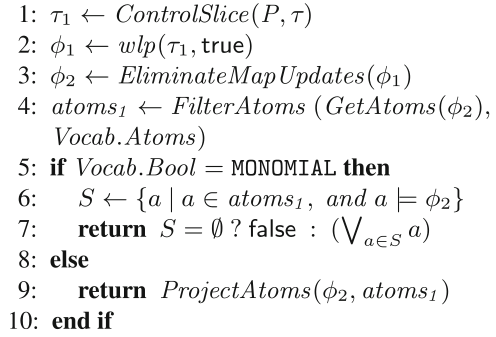
\includegraphics[width=0.9\linewidth]{img/explainErrorShort.png}
%\end{frame}

\begin{frame}{ExplainError}
\begin{algorithmic} \small
\State $\tau^\prime \gets \textit{ControlSlice}(P, \tau)$
\State $\phi_1 \gets \textit{wlp}(\tau^\prime)$
\State $\phi_2 \gets \textit{EliminateMapUpdates}(\phi_1)$
\State $\phi_3 \gets \textit{Simplify}(\phi_2)$

%\If {$\textsc{Permissive}(P_{\emptyset, B}, E \cup \{ \phi \} )$}
%  \State $E \gets E \cup \{ \phi \}$
%\Else
%  \State Let $a$ be the failing assert in $\tau$.
%  \State Remove $a$ from $A^\prime$
%\EndIf
\end{algorithmic}
\end{frame}

\begin{frame}{Shrnutí}

\end{frame}


%% Pomocí shovívavých vstupních podmínek definujeme andělskou korektnost.
%\begin{frame}{Andělská korektnost}
%\begin{dfn}
%Mějme program P obsahující sadu běžných assertů $A$
%a sadu andělských assertů $\hat{A}$, spolu se slovníkem formulí \texttt{Vocab}.
%Říkáme, že P je andělsky korektní za předpokladu $( \texttt{Vocab}, \hat{A} )$,
%pokud existuje formule $\phi \in \textsf{Vocab}$, která je shovívavou vstupní podmínkou programu P,
%a přitom $\phi \vDash P_{A, \emptyset}$. 
%\end{dfn}
%\end{frame}
%
%% Předpokládejme teď, že Vocab je množina všech formulí.
%% a andělská asserty jsou právě asserty uvedené modře.
%% Je tento program andělsky korektní? S jakým předpokladem?
%% Možné podmínky: false, x > 100
%\begin{frame}[fragile]{Je andělsky korektní?}
%Obyčejné asserty černě, andělské asserty \textcolor{blue}{modře}.
%%\setbeamerfont{alerted text}{series=\footnotesize,family=\ttfamily}
%\begin{semiverbatim} \small
%start:
%  \only<2>{\textcolor{blue}{assert x > 5;}}\only<3>{\textcolor{blue}{assert x > 2;}}
%  assert x > 3;
%  goto
%\end{semiverbatim}
%
%
%\end{frame}

%
%\begin{frame}{ExplainError}
%\begin{columns}
%
%% Vygeneruje bud formuli v CNF, nebo jen jednu klauzuli (ryhlejsi)
%\begin{column}{0.5\textwidth}
%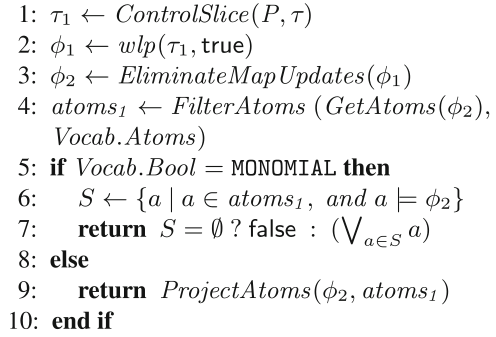
\includegraphics[width=0.9\linewidth]{img/explainErrorShort.png}
%\end{column}
%
%\begin{column}{0.5\textwidth}
%Explanation
%\end{column}
%
%\end{columns}
%\end{frame}

%\begin{frame}{Shrnutí}
%
%\end{frame}
%


\end{document}